\documentclass{article}
\usepackage[UTF8]{ctex} 
\usepackage{amsmath}
\usepackage{bm}
\usepackage{amssymb}
\usepackage{geometry}
\usepackage{graphicx}
\usepackage{listings}
\usepackage{tikz}
\usepackage{amsthm}
\newtheorem{theorem}{定理}
\usetikzlibrary{calc}
\usetikzlibrary{shapes.multipart}
\usetikzlibrary{arrows.meta, positioning, shapes.geometric}
\usetikzlibrary{decorations.pathreplacing, fit}
\geometry{a4paper, margin=1.5cm}

\title{排序技术2}
\author{Tan Yiqing}
\date{\today}

\begin{document}
\maketitle
    
    \begin{figure}[h]
        \centering
        \includegraphics[width=0.75\textwidth]{D:/program/data_construction/firefly/v2-475c384f92fd4a7872be6ae3a93f0b0c_720w.png}
    \end{figure}

\section{交换排序(续)}
\subsection{快速排序(续)}
\subsubsection{快速排序的代码流程}
笔者觉得快排比较重要而且相对比较复杂,所以这里给出代码流程说明。
\begin{lstlisting}[language=C++, caption={快速排序的一次划分过程}]
template <class T>
int quickPivot(T* &arr, int n, int sIndex, int eIndex){ 
    //use first element as pivot, put pivot in correct position, return index
    int le = sIndex;
    int ri = eIndex;
    while(le < ri){
        // 1) 先从右往左找:寻找一个“比左侧当前元素 arr[le] 小”的元素
        while(le < ri && arr[le] <= arr[ri]) ri--;
        //把“小元素”放到左侧区域
        if(le < ri){
            T tmp = arr[le];
            arr[le] = arr[ri];
            arr[ri] = tmp;
            le++;    //左侧“已处理区”扩大
        }
        // 2) 再从左往右找:寻找一个“比右侧当前元素 arr[ri] 大”的元素
        while(le < ri && arr[le] <= arr[ri]) le++;
        //把“大元素”放到右侧区域
        if(le < ri){
            T tmp = arr[le];
            arr[le] = arr[ri];
            arr[ri] = tmp;
            ri--;    //右侧“已处理区”扩大
        }
    }
    return le;
}
\end{lstlisting}

\paragraph{例子演示:}
以数组 $[7,5,8,5,3,4,1,6,2]$ 为例,演示一次 quickPivot 划分过程(枢轴为第一个元素 $7$)。

\begin{center}
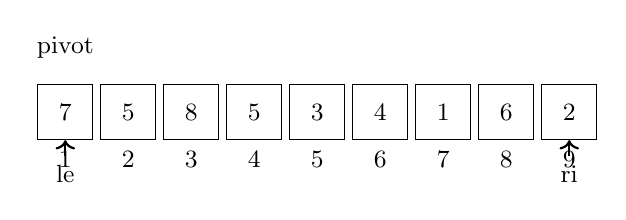
\begin{tikzpicture}[node distance=0.6cm, font=\small]
    % 数组元素
    \foreach \x [count=\i] in {7,5,8,5,3,4,1,6,2} {
        \node[draw, rectangle, minimum width=0.7cm, minimum height=0.7cm] (A\i) at (\i*0.8,0) {\x};
    }
    % 下标
    \foreach \i in {1,...,9} {
        \node at (\i*0.8,-0.6) {\i};
    }
    % le, ri 指针初始
    \node[below=0.2cm of A1] (le) {le};
    \draw[->, thick] (le) -- (A1.south);
    \node[below=0.2cm of A9] (ri) {ri};
    \draw[->, thick] (ri) -- (A9.south);
    % 标注
    \node[above=0.2cm of A1] {pivot};
\end{tikzpicture}

初始状态:le=1,ri=9,pivot=7。
\end{center}

\begin{enumerate}
    \item 从右往左找,直到 $arr[ri] < arr[le]$,找到 $arr[9]=2 < 7$,交换 $arr[1]$ 和 $arr[9]$,数组变为 $[2,5,8,5,3,4,1,6,7]$,le=2。
    \item 从左往右找,直到 $arr[le] > arr[ri]$,le 依次移动到 $arr[3]=8 > 7$,交换 $arr[3]$ 和 $arr[9]$,数组变为 $[2,5,7,5,3,4,1,6,8]$,ri=8。
    \item 从右往左找,直到 $arr[ri]=6 < 7$,交换 $arr[3]$ 和 $arr[8]$,数组变为 $[2,5,6,5,3,4,1,7,8]$,le=4。
    \item 从左往右找,le 移动到 $arr[7]=1 < 7$,le=8。
    \item le=ri=8,划分结束,pivot $7$ 已到正确位置。
\end{enumerate}

\begin{center}
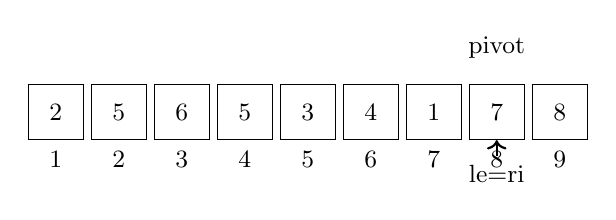
\begin{tikzpicture}[node distance=0.6cm, font=\small]
    % 数组元素
    \foreach \x [count=\i] in {2,5,6,5,3,4,1,7,8} {
        \node[draw, rectangle, minimum width=0.7cm, minimum height=0.7cm] (B\i) at (\i*0.8,0) {\x};
    }
    % 下标
    \foreach \i in {1,...,9} {
        \node at (\i*0.8,-0.6) {\i};
    }
    % le, ri 指针最终
    \node[below=0.2cm of B8] (le2) {le=ri};
    \draw[->, thick] (le2) -- (B8.south);
    % 标注
    \node[above=0.2cm of B8] {pivot};
\end{tikzpicture}

最终状态:pivot $7$ 已到正确位置(第8位)。
\end{center}



\subsubsection{快速排序的性能分析}
\paragraph{时间复杂度} 分析如下:
\begin{enumerate}
    \item \textbf{最好情况:}每一次划分对一个记录定位后,该记录的左侧子表与右侧子表的长度相同,为$O(n\log_2 n)$。
    \[
        T(n) \leq 2T\left(\frac{n}{2}\right) + n
    \]
    展开递推式如下:
    \[
        \begin{aligned}
        T(n) &\leq 2T\left(\frac{n}{2}\right) + n \\
            &\leq 2\left[2T\left(\frac{n}{4}\right) + \frac{n}{2}\right] + n = 4T\left(\frac{n}{4}\right) + 2n \\
            &\leq 4\left[2T\left(\frac{n}{8}\right) + \frac{n}{4}\right] + 2n = 8T\left(\frac{n}{8}\right) + 3n \\
            &\quad \cdots \\
            &\leq nT(1) + n\log_2 n = O(n\log_2 n)
        \end{aligned}
    \]
    上述递推式表示:每一层递归都将问题规模减半,并且每层需要 $O(n)$ 的比较和移动操作。
    递归的层数为 $\log_2 n$,每层总操作量为 $n$,因此总的时间复杂度为 $O(n\log_2 n)$。
    
    \item \textbf{最坏情况:}
    每次划分只得到一个比上一次划分少一个记录的子序列(另一个子序列为空),为 $O(n^2)$。
    \[
        \Sigma_{i=1}^{n-1} n-i = \frac{n(n-1)}{2} = O(n^2)
    \]
    一个反直觉的事情是最坏情况的典型例子是正序和反序!

    \item \textbf{平均情况:}时间复杂度为 $O(n\log_2 n)$。
\end{enumerate}

\section{选择排序(selection sort)}
\indent 选择排序的主要操作是选择,其主要思想是:
每趟排序在当前待排序序列中选出关键码最小的记录,添加到有序序列中。

\vspace{4cm}

\begin{center}
% 第1轮
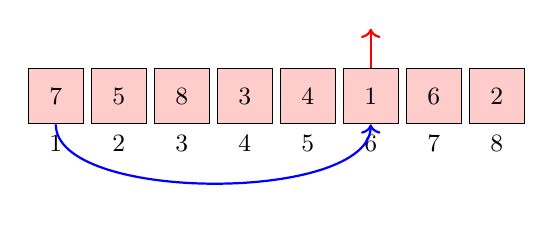
\begin{tikzpicture}[node distance=0.6cm, font=\small]
    % 原始数组,未排序区红色
    \foreach \x [count=\i] in {7,5,8,3,4,1,6,2} {
        \node[draw, rectangle, minimum width=0.7cm, minimum height=0.7cm, fill=red!20] (A\i) at (\i*0.8,0) {\x};
    }
    % 下标
    \foreach \i in {1,...,8} {
        \node at (\i*0.8,-0.6) {\i};
    }
    % 最小值箭头
    \draw[->, thick, red] (A6.north) -- ++(0,0.5);
    % 交换箭头
    \draw[->, thick, blue] (A1.south) .. controls +(0,-1) and +(0,-1) .. (A6.south);
\end{tikzpicture}

% 第1轮后
\begin{tikzpicture}[node distance=0.6cm, font=\small]
    % 有序区绿色,未排序区红色
    \node[draw, rectangle, minimum width=0.7cm, minimum height=0.7cm, fill=green!30] (B1) at (0.8,0) {1};
    \foreach \x [count=\i] in {5,8,3,4,7,6,2} {
        \node[draw, rectangle, minimum width=0.7cm, minimum height=0.7cm, fill=red!20] (B\i) at (\i*0.8+0.8,0) {\x};
    }
    % 下标
    \foreach \i in {1,...,8} {
        \node at (\i*0.8,-0.6) {\i};
    }
    % 最小值箭头
    \draw[->, thick, red] (B8.north) -- ++(0,0.5);
    % 交换箭头
    \draw[->, thick, blue] (B2.south) .. controls +(0,-1) and +(0,-1) .. (B8.south);
\end{tikzpicture}

% 第2轮后
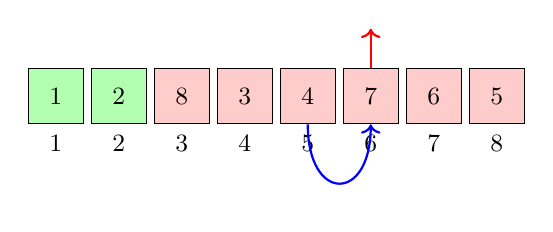
\begin{tikzpicture}[node distance=0.6cm, font=\small]
    % 有序区绿色,未排序区红色
    \node[draw, rectangle, minimum width=0.7cm, minimum height=0.7cm, fill=green!30] (C1) at (0.8,0) {1};
    \node[draw, rectangle, minimum width=0.7cm, minimum height=0.7cm, fill=green!30] (C2) at (1.6,0) {2};
    \foreach \x [count=\i] in {8,3,4,7,6,5} {
        \node[draw, rectangle, minimum width=0.7cm, minimum height=0.7cm, fill=red!20] (C\i) at (\i*0.8+1.6,0) {\x};
    }
    % 下标
    \foreach \i in {1,...,8} {
        \node at (\i*0.8,-0.6) {\i};
    }
    % 最小值箭头
    \draw[->, thick, red] (C4.north) -- ++(0,0.5);
    % 交换箭头
    \draw[->, thick, blue] (C3.south) .. controls +(0,-1) and +(0,-1) .. (C4.south);
\end{tikzpicture}

\vspace{0.1cm}

% 第3轮后
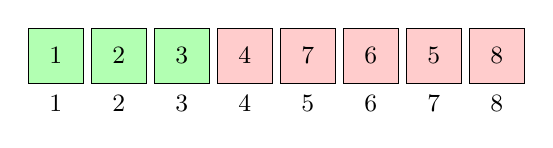
\begin{tikzpicture}[node distance=0.6cm, font=\small]
    % 有序区绿色,未排序区红色
    \node[draw, rectangle, minimum width=0.7cm, minimum height=0.7cm, fill=green!30] (D1) at (0.8,0) {1};
    \node[draw, rectangle, minimum width=0.7cm, minimum height=0.7cm, fill=green!30] (D2) at (1.6,0) {2};
    \node[draw, rectangle, minimum width=0.7cm, minimum height=0.7cm, fill=green!30] (D3) at (2.4,0) {3};
    \foreach \x [count=\i] in {4,7,6,5,8} {
        \node[draw, rectangle, minimum width=0.7cm, minimum height=0.7cm, fill=red!20] (D\i) at (\i*0.8+2.4,0) {\x};
    }
    % 下标
    \foreach \i in {1,...,8} {
        \node at (\i*0.8,-0.6) {\i};
    }
\end{tikzpicture}
\end{center}


\subsection{性能分析}
\paragraph{时间复杂度} 分析如下:
\begin{enumerate}
    \item 最好情况:
    \begin{enumerate}
        \item 比较次数:$\frac{n(n-1)}{2}$次。
        \item 移动次数:$0$次。
    \end{enumerate}
    时间复杂度为$O(n^2)$。
    \item 最坏情况:
    \begin{enumerate}
        \item 比较次数:$\frac{n(n-1)}{2}$次。
        \item 移动次数:$3(n-1)$次。
    \end{enumerate}
    时间复杂度为$O(n^2)$。
    \item 平均情况:时间复杂度为$O(n^2)$。
\end{enumerate}

\paragraph{空间复杂度} 需要一个辅助空间存放临时变量,空间复杂度为$O(1)$。

\paragraph{稳定性} 选择排序是\pmb{不稳定}的排序算法!
反例:对[(f,1),(b,2),(c,3),(f,4),(a,1)]进行选择排序,第一次选择后得到[(a,1),(b,2),(c,3),(f,4),(f,1)],两个(f,1)和(f,4)的相对位置发生了改变。

\subsection{改进方法}
\indent 关键在于减少关键码的比较次数,可以采用\textbf{堆排序}来实现选择排序的改进。

\subsubsection{堆的定义}
\pmb{堆}是具有下列性质的完全二叉树:每个结点的值都小于或等于其左右孩子结点的值(称为小根堆),或每个结点的值都大于或等于其左右孩子结点的值(称为大根堆)。

\begin{center}
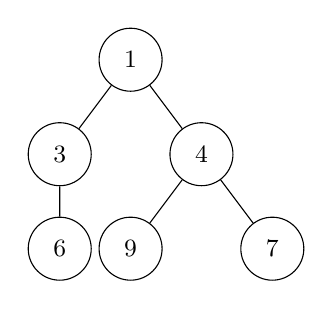
\begin{tikzpicture}[level distance=1.2cm, sibling distance=1.8cm, every node/.style={draw, circle, minimum size=0.8cm, font=\small}]
  \node {1}
    child {node {3}
      child {node {6}}
    }
    child {node {4}
      child {node {9}}
      child {node {7}}
    };
\end{tikzpicture}
\end{center}

\indent 小根堆的根结点是所有结点的最小者。较小结点靠近根结点,但不绝对。(大根堆反之)

\indent 堆采用顺序结构存储,比如上面可以用层序存储为数组 $[1,3,4,6,9,7]$。

\subsubsection{基本思想与代码实现}
首先将待排序的记录序列构造成一个堆,此时,选出了堆中所有记录的\pmb{最大者},然后将它从堆中移走,
并将剩余的记录再调整成堆,这样又找出了\pmb{次小的记录},以此类推,直到堆中只有一个记录。\\
\indent 所以,问题来到如何\pmb{构造堆}和\pmb{调整堆}。

\paragraph{堆构造}
\begin{enumerate}
    \item 从最后一个非叶节点开始,依次向上对每个节点进行“向下调整”。
    \item 每次调整时,将当前节点与其左右孩子中较小者比较,若孩子更小则交换,并递归对子节点继续调整。
    \item 重复上述过程,直到根节点也调整完毕,整个序列就变成了一个堆。
\end{enumerate}

假设初始无序序列为 $[4,7,6,3,1,8]$,其完全二叉树结构如下:

\begin{center}
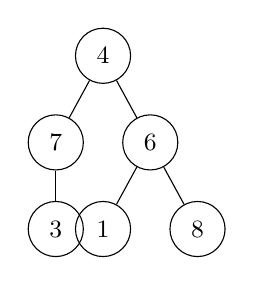
\begin{tikzpicture}[level distance=1.1cm, sibling distance=1.2cm, every node/.style={draw, circle, minimum size=0.7cm, font=\small}]
\node {4}
  child {node {7}
    child {node {3}}
  }
  child {node {6}
    child {node {1}}
    child {node {8}}
  };
\end{tikzpicture}
\end{center}

\textbf{步骤1:从最后一个非叶节点(7)开始向下调整。}

7的左孩子为3,比7小,交换7和3。

\begin{center}
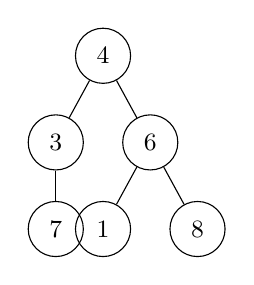
\begin{tikzpicture}[level distance=1.1cm, sibling distance=1.2cm, every node/.style={draw, circle, minimum size=0.7cm, font=\small}]
\node {4}
  child {node {3}
    child {node {7}}
  }
  child {node {6}
    child {node {1}}
    child {node {8}}
  };
\end{tikzpicture}
\end{center}

\textbf{步骤2:向上回到根节点(4),向下调整。}

4的左孩子为3,右孩子为6,3最小,交换4和3。

\begin{center}
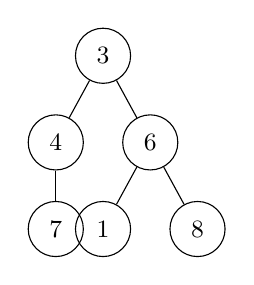
\begin{tikzpicture}[level distance=1.1cm, sibling distance=1.2cm, every node/.style={draw, circle, minimum size=0.7cm, font=\small}]
\node {3}
  child {node {4}
    child {node {7}}
  }
  child {node {6}
    child {node {1}}
    child {node {8}}
  };
\end{tikzpicture}
\end{center}

\textbf{步骤3:继续调整4的子树。}

4的左孩子为7,右孩子为空,无需调整。

\textbf{步骤4:调整右子树(6)。}

6的左孩子为1,比6小,交换6和1。

\begin{center}
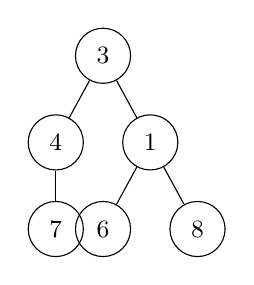
\begin{tikzpicture}[level distance=1.1cm, sibling distance=1.2cm, every node/.style={draw, circle, minimum size=0.7cm, font=\small}]
\node {3}
  child {node {4}
    child {node {7}}
  }
  child {node {1}
    child {node {6}}
    child {node {8}}
  };
\end{tikzpicture}
\end{center}

\textbf{步骤5:回到根节点,检查是否需要继续调整。}

根节点3的左右孩子为4和1,1最小,交换3和1。

\begin{center}
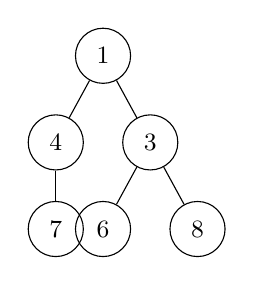
\begin{tikzpicture}[level distance=1.1cm, sibling distance=1.2cm, every node/.style={draw, circle, minimum size=0.7cm, font=\small}]
\node {1}
  child {node {4}
    child {node {7}}
  }
  child {node {3}
    child {node {6}}
    child {node {8}}
  };
\end{tikzpicture}
\end{center}

\textbf{最终得到小根堆结构。}

\paragraph{堆调整} 在一棵完全二叉树中,根结点的左右子树均是堆,如何调整根结点,使整个完全二叉树成为一个堆?

\begin{center}
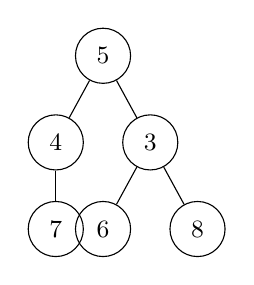
\begin{tikzpicture}[level distance=1.1cm, sibling distance=1.2cm, every node/.style={draw, circle, minimum size=0.7cm, font=\small}]
\node {5}
  child {node {4}
    child {node {7}}
  }
  child {node {3}
    child {node {6}}
    child {node {8}}
  };
\end{tikzpicture}
\end{center}

\noindent
此时,根节点5大于右孩子3,需要与3交换,调整如下:

\begin{center}
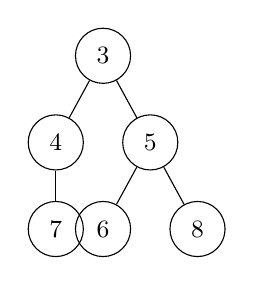
\begin{tikzpicture}[level distance=1.1cm, sibling distance=1.2cm, every node/.style={draw, circle, minimum size=0.7cm, font=\small}]
\node {3}
  child {node {4}
    child {node {7}}
  }
  child {node {5}
    child {node {6}}
    child {node {8}}
  };
\end{tikzpicture}
\end{center}

\noindent
继续对5进行向下调整。5的左孩子为6,右孩子为8,5已经小于它们,无需再调整,最终得到小根堆:

\begin{center}
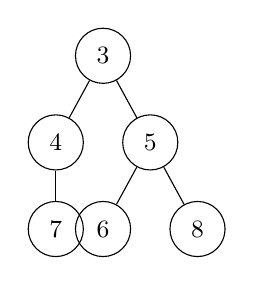
\begin{tikzpicture}[level distance=1.1cm, sibling distance=1.2cm, every node/.style={draw, circle, minimum size=0.7cm, font=\small}]
\node {3}
  child {node {4}
    child {node {7}}
  }
  child {node {5}
    child {node {6}}
    child {node {8}}
  };
\end{tikzpicture}
\end{center}

\noindent
\textbf{总结:}只需将根节点与左右子树中较小的根交换,并递归对子树调整,即可使整棵树成为堆。

以上过程都是在二叉树上的可视化,如何在顺序结构上实现呢?先给出如下的对应关系:
\begin{enumerate}
    \item 堆构建:\\
    for (i=n/2; i>=1; i--)
        sift(r, i, n) ; 
    \item 堆调整:\\
    sift(r, i, n): 
    \item 处理堆顶记录:\\
    swap(r[1], r[n]) ;
\end{enumerate}

\begin{lstlisting}[language=C++, caption={堆排序的顺序结构实现}]
/* 向下调整,使以i为根的子树成为小根堆 */
void sift(int r[], int i, int n) {
    int tmp = r[i];
    int child = 2 * i;
    while (child <= n) {
        // 选出左右孩子中较小的
        if (child + 1 <= n && r[child + 1] < r[child]) {
            child++;
        }
        if (r[child] < tmp) {
            r[i] = r[child];
            i = child;
            child = 2 * i;
        } else {
            break;
        }
    }
    r[i] = tmp;
}

/* 堆排序主过程 */
void heapSort(int r[], int n) {
    // 1. 堆构建(下标从1开始)
    for (int i = n / 2; i >= 1; i--) {
        sift(r, i, n);
    }
    // 2. 反复取堆顶元素放到末尾,并调整堆
    for (int i = n; i > 1; i--) {
        swap(r[1], r[i]); // 处理堆顶记录
        sift(r, 1, i - 1); // 堆调整
    }
}
\end{lstlisting}

\subsubsection{堆排序性能分析}
\paragraph{时间复杂度} 分析如下:
\begin{enumerate}
    \item 第一个for是堆构造:$O(n)$。
    \item 第二个for是输出堆顶重建堆,共需要取n-1次堆顶记录,
    第 i 次取堆顶记录重建堆需要$O(\log_2 i)$时间,所以需要$O(n\log_2 n)$时间;
\end{enumerate}
因此整个堆排序的时间复杂度为$O(n\log_2 n)$,这是堆排序的最好、最坏和平均的时间代价。


\section{归并排序(mergesort)}
\pmb{归并}是指将两个或两个以上的有序序列合并成一个有序序列的过程。 \\
\indent 归并排序的主要操作是归并,其主要思想是:将若干有序序列逐步归并,最终得到一个有序序列。
\subsection{二路归并排序}
将一个具有n个待排序记录的序列看成是n个长度为1的有序序列,然后进行两两归并,得到n/2个长度为2的有序序列,
再进行两两归并,得到n/4个长度为4的有序序列,以此类推,直至得到一个长度为n的有序序列为止。

\begin{center}
\textbf{二路归并排序过程示意图}

\begin{tikzpicture}[node distance=0.6cm, font=\small]
    % 原始序列
    \foreach \x [count=\i] in {7, 5, 8, 3, 4, 1, 6, 2} {
        \node[draw, rectangle, minimum width=0.7cm, minimum height=0.7cm] (A\i) at (\i*0.9,0) {\x};
    }
    \node at (0.9*4.5, -0.7) {初始序列};

    % 第一轮归并
    \foreach \i/\j in {1/2, 3/4, 5/6, 7/8} {
        \draw[->, thick, blue] (A\i.south) -- ++(0,-0.5) -| (A\j.south);
    }
    \foreach \i [count=\k from 1] in {5,7,3,8,1,4,2,6} {
        \node[draw, rectangle, minimum width=0.7cm, minimum height=0.7cm, fill=blue!10] (B\k) at (\k*0.9,-1.5) {\i};
    }

    % 第二轮归并
    \foreach \i/\j in {1/2, 3/4, 5/6, 7/8} {
        \draw[->, thick, green!60!black] (B\i.south) -- ++(0,-0.5) -| (B\j.south);
    }
    \foreach \i [count=\k from 1] in {3,5,7,8,1,2,4,6} {
        \node[draw, rectangle, minimum width=0.7cm, minimum height=0.7cm, fill=green!10] (C\k) at (\k*0.9,-3) {\i};
    }

    % 第三轮归并
    \draw[->, thick, red] (C1.south) -- ++(0,-0.5) -| (C4.south);
    \draw[->, thick, red] (C5.south) -- ++(0,-0.5) -| (C8.south);
    \foreach \i [count=\k from 1] in {1,2,3,4,5,6,7,8} {
        \node[draw, rectangle, minimum width=0.7cm, minimum height=0.7cm, fill=red!10] (D\k) at (\k*0.9,-4.5) {\i};
    }

    % 标签
    \node at (-0.5, 0) {第0轮};
    \node at (-0.5, -1.5) {第1轮};
    \node at (-0.5, -3) {第2轮};
    \node at (-0.5, -4.5) {第3轮};
\end{tikzpicture}
\end{center}

\noindent 在归并过程中,可能会破坏原来的有序序列,所以,将归并的结果存入另外一个数组中。

\subsection{伪代码}
\begin{lstlisting}[language=C++, caption={二路归并排序伪代码}]
void MergeSort2(int r[ ], int r1[ ], int s, int t)
{ 
    if (s==t) r1[s]=r[s];                 //递归出口,用有序长度来控制
    else { 
         m=(s+t)/2;
         MergeSort2(r, r1, s, m);           //归并排序前半个子序列
         MergeSort2(r, r1, m+1, t);       //归并排序后半个子序列
         Merge(r1, r, s, m, t);           将两个已排序的子序列归并
    }
}
\end{lstlisting}

\subsection{性能分析}
\begin{enumerate}
    \item 时间复杂度:一趟归并操作是将r[1]~r[n]中相邻的长度为h的有序序列进行两两归并,并把结果存放到r1[1]~r1[n]中,这需要$O(n)$时间。
    整个归并排序需要进行趟$\lceil \log_2 n \rceil$,因此,总的时间代价是$O(n\log_2 n)$。这是归并排序算法的最好、最坏、平均的时间性能。
    \item 空间复杂度:算法在执行时,需要占用与原始记录序列同样数量的存储空间,因此空间复杂度为$O(n)$。
\end{enumerate}

\section{分配排序(distribution sort)}
\pmb{桶}是指一个用于临时存放数据的容器。\\
\indent 分配排序是基于分配和收集的排序方法,其基本思想是:先将待排序记录序列分配到不同的桶里,然后再把各桶中的记录依次收集到一起。 

\subsection{桶排序(bucket sort)}
假设待排序记录的值都在0~m-1之间,设置m个桶,首先将值为i的记录分配到第i个桶中,然后再将各个桶中的记录依次收集起来。\\
\indent 实际写的使用,用静态链队列来实现每个桶是个不错的选择。

\begin{center}
\textbf{桶排序过程示意图}

\begin{tikzpicture}[node distance=0.6cm, font=\small]
    % 原始序列
    \node at (0,0.8) {原始序列:};
    \foreach \x [count=\i] in {2, 4, 3, 2, 1, 0, 4, 3, 1, 0} {
        \node[draw, rectangle, minimum width=0.7cm, minimum height=0.7cm] (A\i) at (\i*0.9,0) {\x};
    }

    % 箭头到桶
    \foreach \i/\val in {1/2, 2/4, 3/3, 4/2, 5/1, 6/0, 7/4, 8/3, 9/1, 10/0} {
        \draw[->, thick] (A\i.south) -- ++(0,-0.5) -| (\val*2.2-0.5,-2.2);
    }

    % 桶
    \foreach \i in {0,1,2,3,4} {
        \node[draw, rectangle, minimum width=1.2cm, minimum height=1.2cm, fill=blue!10] (B\i) at (\i*2.2-0.5,-2.2) {};
        \node at (\i*2.2-0.5,-3.1) {桶\i};
    }
    % 桶内元素
    \node at (-0.5,-2.2) {0,0};
    \node at (1.7,-2.2) {1,1};
    \node at (3.9,-2.2) {2,2};
    \node at (6.1,-2.2) {3,3};
    \node at (8.3,-2.2) {4,4};

    % 收集箭头
    \foreach \i in {0,1,2,3,4} {
        \draw[->, thick, red] (B\i.south) -- ++(0,-0.7) -- ++(0.5,-0.2);
    }
    % 有序序列
    \node at (0,-4.2) {有序序列:};
    \foreach \x [count=\i] in {0,0,1,1,2,2,3,3,4,4} {
        \node[draw, rectangle, minimum width=0.7cm, minimum height=0.7cm, fill=green!10] (C\i) at (\i*0.9,-5) {\x};
    }
\end{tikzpicture}
\end{center}

\subsubsection{桶排序性能分析}
\begin{enumerate}
    \item \textbf{时间复杂度:}假定用一个静态链表存储所有桶,用静态链队列实现桶。
    桶式排序第一个循环初始化静态链表,时间性能为$O(n)$,
    第二个循环初始化静态链队列,时间性能为$O(m)$,
    进行分配需要遍历静态链表,时间性能为$O(n)$,
    进行收集需要遍历静态链表和静态链队列,因此,桶式排序的时间复杂度为$O(n + m)$。
    \item \textbf{空间复杂度:}桶式排序的空间复杂度是$O(m)$,用来存储m个静态队列表示的桶。
    \item \textbf{稳定性:}桶排序是\pmb{稳定}的排序算法。
\end{enumerate}

\subsection{基数排序(radix sort)}
基本思想是:将关键码看成由若干个子关键码复合而成,然后借助分配和收集操作。具体来说:

\begin{enumerate}
    \item 第1趟排序:按最低位关键码 $kd-1$ 将具有相同码值的记录分配到一个队列(桶)中,然后依次收集起来,得到一个按关键码 $kd-1$ 有序的序列;
    \item 第$i$趟排序:按关键码 $kd-i$ 将具有相同码值的记录分配到一个队列(桶)中,然后依次收集起来,得到一个按关键码 $kd-i$ 有序的序列。
\end{enumerate}

\indent 上面是PPT上的,人话的话可以举个例子:先把个位一样的放一起,再把十位一样的放一起……

\vspace{5cm}

\begin{center}
\textbf{基数排序完整流程示意图}

\begin{tikzpicture}[node distance=0.6cm, font=\small]
    % 原始序列
    \node at (0,1.2) {原始序列:};
    \foreach \x [count=\i] in {421, 240, 035, 532, 305, 430, 124, 233} {
        \node[draw, rectangle, minimum width=1.1cm, minimum height=0.7cm] (A\i) at (\i*1.2,0) {\x};
    }

    % 第1趟:个位分配
    \foreach \i/\val in {1/1, 2/0, 3/5, 4/2, 5/5, 6/0, 7/4, 8/3} {
        \draw[->, thick] (A\i.south) -- ++(0,-0.5) -| (\val*2.0-1.5,-2.2);
    }
    % 个位桶
    \foreach \i in {0,1,2,3,4,5} {
        \node[draw, rectangle, minimum width=1.5cm, minimum height=1.2cm, fill=blue!10] (B\i) at (\i*2.0-1.5,-2.2) {};
        \node at (\i*2.0-1.5,-3.1) {桶\i};
    }
    % 桶内元素(个位)
    \node at (-1.5,-2.2) {240, 430};
    \node at (0.5,-2.2) {421};
    \node at (2.5,-2.2) {532};
    \node at (4.5,-2.2) {233};
    \node at (6.5,-2.2) {124};
    \node at (8.5,-2.2) {035, 305};

    % 收集箭头
    \foreach \i in {0,1,2,3,4,5} {
        \draw[->, thick, red] (B\i.south) -- ++(0,-0.7) -- ++(0.5,-0.2);
    }
    % 第1趟后序列
    \node at (0,-4.2) {第1趟后:};
    \foreach \x [count=\i] in {240,430,421,532,233,124,035,305} {
        \node[draw, rectangle, minimum width=1.1cm, minimum height=0.7cm, fill=green!10] (C\i) at (\i*1.2,-5) {\x};
    }

    % 第2趟:十位分配
    \foreach \i/\val in {1/4, 2/3, 3/2, 4/3, 5/3, 6/2, 7/3, 8/0} {
        \draw[->, thick, orange] (C\i.south) -- ++(0,-0.5) -| (\val*2.0-1.5,-7.2);
    }
    % 十位桶
    \foreach \i in {0,1,2,3,4,5} {
        \node[draw, rectangle, minimum width=1.5cm, minimum height=1.2cm, fill=orange!10] (D\i) at (\i*2.0-1.5,-7.2) {};
        \node at (\i*2.0-1.5,-8.1) {桶\i};
    }
    % 桶内元素(十位)
    \node at (-1.5,-7.2) {305};
    \node at (0.5,-7.2) {};
    \node at (2.5,-7.2) {240,124};
    \node at (4.5,-7.2) {430,421,532,233};
    \node at (6.5,-7.2) {};
    \node at (8.5,-7.2) {035};

    % 收集箭头
    \foreach \i in {0,1,2,3,4} {
        \draw[->, thick, red] (D\i.south) -- ++(0,-0.7) -- ++(0.5,-0.2);
    }
    % 第2趟后序列
    \node at (0,-9.2) {第2趟后:};
    \foreach \x [count=\i] in {305,240,124,430,421,532,233,035} {
        \node[draw, rectangle, minimum width=1.1cm, minimum height=0.7cm, fill=yellow!10] (E\i) at (\i*1.2,-10) {\x};
    }

    % 第3趟:百位分配
    \foreach \i/\val in {1/3, 2/2, 3/1, 4/4, 5/4, 6/5, 7/2, 8/0} {
        \draw[->, thick, purple] (E\i.south) -- ++(0,-0.5) -| (\val*2.0-1.5,-12.2);
    }
    % 百位桶
    \foreach \i in {0,1,2,3,4,5} {
        \node[draw, rectangle, minimum width=1.5cm, minimum height=1.2cm, fill=purple!10] (F\i) at (\i*2.0-1.5,-12.2) {};
        \node at (\i*2.0-1.5,-13.1) {桶\i};
    }
    % 桶内元素(百位)
    \node at (-1.5,-12.2) {035};
    \node at (0.5,-12.2) {124};
    \node at (2.5,-12.2) {240,233};
    \node at (4.5,-12.2) {305, 430, 421};
    \node at (6.5,-12.2) {532};

    % 收集箭头
    \foreach \i in {0,1,2,3,4,5} {
        \draw[->, thick, red] (F\i.south) -- ++(0,-0.7) -- ++(0.5,-0.2);
    }
    % 最终有序序列
    \node at (0,-14.2) {最终有序:};
    \foreach \x [count=\i] in {035,124,233,240,305, 421, 430, 532} {
        \node[draw, rectangle, minimum width=1.1cm, minimum height=0.7cm, fill=green!20] (G\i) at (\i*1.2,-15) {\x};
    }
\end{tikzpicture}
\end{center}

\noindent
如上图所示,基数排序每一趟都按对应位分配到桶中,再收集起来,经过所有关键码位的分配与收集后,最终得到有序序列。

\subsubsection{基数排序性能分析}
\begin{enumerate}
    \item \textbf{时间复杂度:}假设待排序记录的关键码由d个子关键码复合而成,每个子关键码的取值范围为m个,则基数排序的时间复杂度为$O(d(n+m))$,其中每一趟分配的时间复杂度是$O(n)$,每一趟收集的时间复杂度为$O(n+m)$,整个排序需要执行d趟。
    \item \textbf{空间复杂度:}基数排序共需要m个队列,因此空间复杂度为$O(m)$。
    \item \textbf{稳定性:}由于桶采用队列作为存储结构,基数排序是\pmb{稳定}的排序算法。
\end{enumerate}


\section{总结}
    
    \begin{figure}[h]
        \centering
        \includegraphics[width=0.75\textwidth]{D:/program/data_construction/L8/理论/搜狗截图20251222180506.png}
    \end{figure}

    \begin{figure}[h]
        \centering
        \includegraphics[width=0.60\textwidth]{D:/program/data_construction/L8/理论/搜狗截图20251222180526.png}
    \end{figure}

    \begin{figure}[h]
        \centering
        \includegraphics[width=0.75\textwidth]{D:/program/data_construction/L8/理论/搜狗截图20251222180539.png}
    \end{figure}

\end{document}